\chapter{Methodology}

\section{Collecting Data: OONI}

\subsection{Background}
Released under the TOR project in 2012, the Open Observatory of Network Interference (OONI) is a non-profit open-source software project whose goal is to empower decentralized efforts to document internet censorship worldwide \cite{OONIAbout}. The OONI organization openly publishes measurements and provides a public archive of network interference across the globe. This has produced a database of more than 2.6 billion individual tests. \cite{OONIExplorer}

OONI data has been used extensively by third parties both for research and advocacy. Examples include the Freedom on the Net 2024 \cite{freedomhouse2024struggle} report, iMAP reports \cite{ooni2024imap} by Sinar, and Access Now’s annual \#KeepItOn 2023 Report. \cite{accessnow2023keepiton} \cite{ooni2024yearinreview} Based on these high profile endorsements and the wealth of data available, OONI is a perfect tool to measure internet censorship.

\subsection{OONI Probe}
Released in 2017, the OONI Probe is a mobile app and software designed to test internet censorship. Users can install and run this software, contributing to the growing dataset in the OONI database. OONI's mission is to \textit{“ensure a free and open internet by increasing transparency of internet censorship worldwide.”} While no user appears to have faced repercussions from using the OONI probe, this may lead to a false sense of security or incorrect assumptions about anonymity. As emphasized in OONI’s onboarding quiz, probe tests can be visible on the network.

The OONI Probe CLI v3.24.0 was used during testing as it is the most recent stable release. Its documentation can be found on GitHub \cite{oonicli2024}.

\subsection{Virtual Machine}
In order to gather ground truth, a virtual machine in Israel is used to run OONI command line interface locally. This machine is accessed via SSH. These technologies will be discussed further below. The chosen provider, \textit{interhost.co.il}, has a strong track record regarding data integrity and security; however, further scrutiny is necessary. \cite{interhost} 

These tools were audited for any security and privacy concerns and the results are below. Tools like CloudFlare's TCP reset dashboard \cite{cloudflare_policy_blog} gave further insight on instances of throttling, blocking or otherwise. In order to expand the web connectivity tests included with OONI, resources like Citizen Lab's sensitive domain list were included. \cite{citizenlab_testlists} 

\section{Ground Truth: Ireland \& Israel}
To gather ground truth in Ireland, the OONI probe Command Line Interface was installed and ran over a two week period. Since the CLI is not natively supported on Windows, a Unix-based operating system was flashed onto a Raspberry Pi 5, which served as a dedicated headless testing device. The device was accessed remotely via SSH, enabling the automation and management of tests. 

\begin{figure} [H]
    \centering
    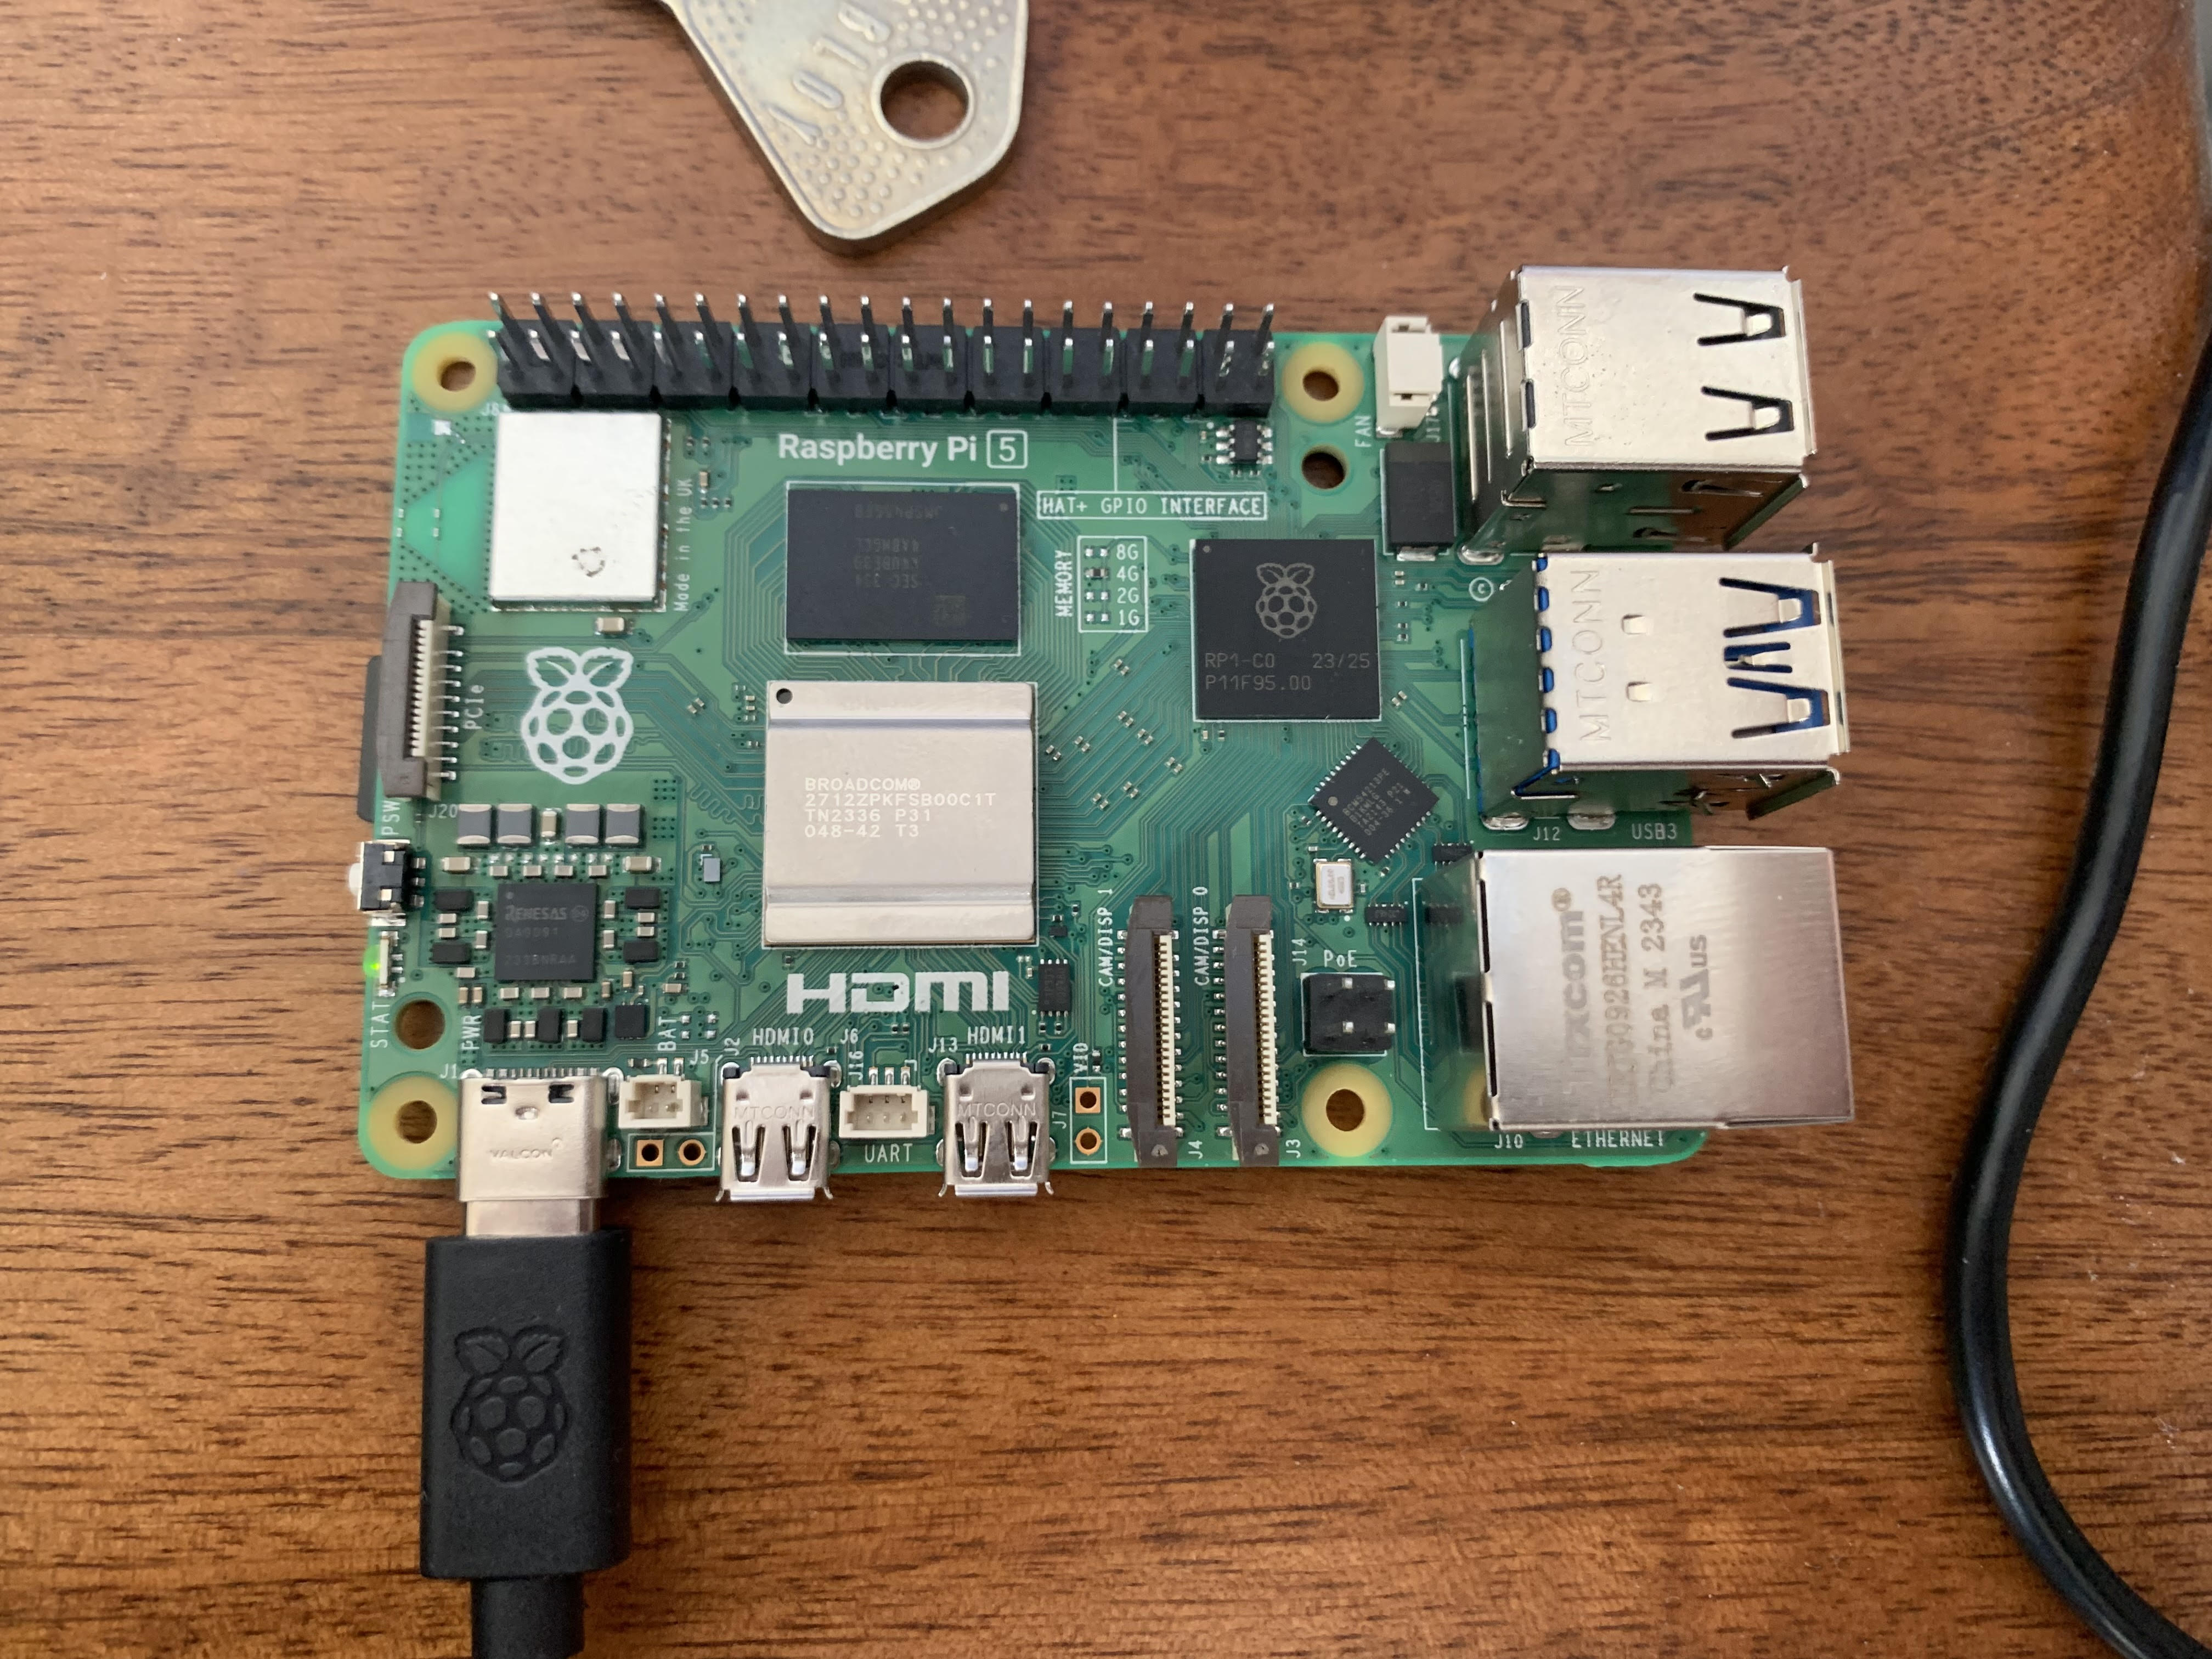
\includegraphics[width=0.5\linewidth]{RasPi5.jpg}
    \caption{Headless Raspberry Pi 5}
    \label{fig:enter-label}
\end{figure}

A similar process was used to remotely control the Israeli VM. This allowed for side-by-side running of tests and comparison of results. 

\begin{figure} [H]
    \centering
    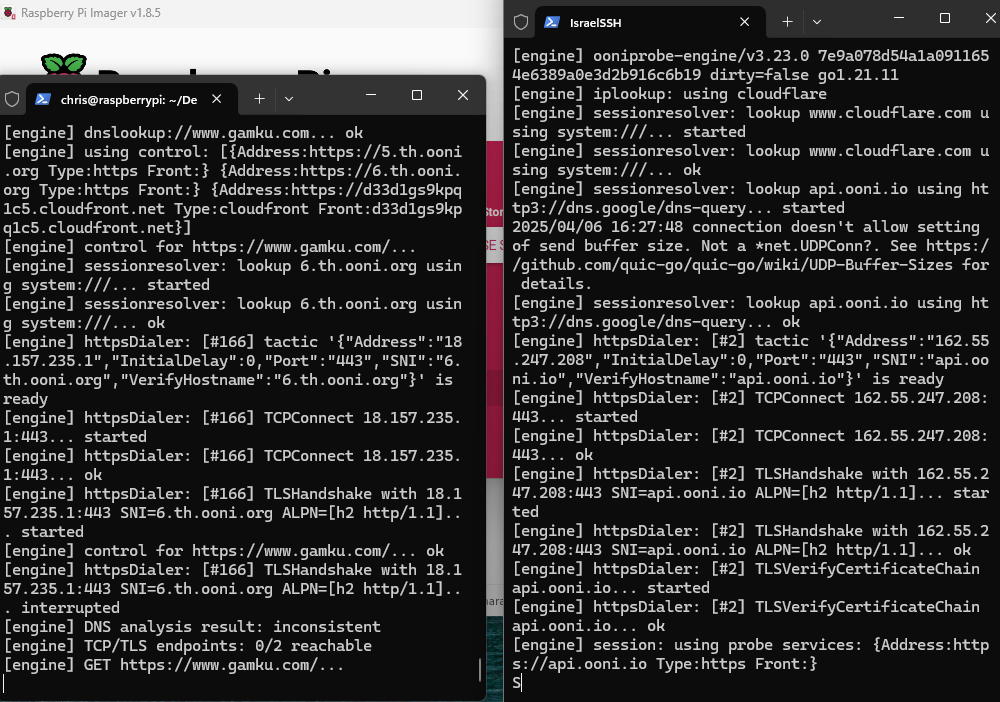
\includegraphics[width=0.5\linewidth]{RunningTestsSideBySideSSH.png}
    \caption{Running OONI tests over SSH}
    \label{fig:enter-label}
\end{figure}

\subsection{Description of OONI Tests}
\subsubsection{Web Connectivity Test}

The Web Connectivity test determines if, and how, access to a specific website may be blocked. To do this, OONI Probe performs several checks from the network where the test is run and compares the results with measurements collected from a control network where censorship is not expected. If the measurements differ significantly, censorship techniques are likely used on the local network. This test is designed to perform the four different actions: Resolver Identification, DNS Lookup, TCP Connect, HTTP GET Request.

The Web Connectivity test begins by identifying the DNS resolver in use on the network. It achieves this by sending DNS queries to special domains, which disclose the resolver’s IP address. Once the resolver is identified, the test performs DNS lookups to determine which IP addresses (and potentially other host names) are mapped to the tested domain. After collecting that information, the test attempts to establish a TCP session on port 80 or port 443, depending on whether the URL uses HTTP or HTTPS. Finally, once the TCP connection is successful, the test sends an HTTP GET request to the server hosting the website; under normal circumstances, the server will respond with the requested webpage content \cite{ooniConnectivityTest}.

\subsubsection{Circumvention Test}

The circumvention test is used to check weather Psiphon, Tor, or RiseupVPN are blocked on a given network. These are tools used to circumvent censorship by utilizing VPN, SSH, and HTTP proxy technologies. 

The Psiphon VPN serves as a tunnel that enables you to circumvent censorship by connected you to an uncensored portion of the internet \cite{ooniPsiphonTest}. The Psiphon test first uses Psiphon’s own code to establish a Psiphon tunnel. After the tunnel is created, the test attempts to load a webpage to see if Psiphon actually works for accessing the internet. If the tunnel is successfully set up and the webpage loads, Psiphon is functioning on the tested network and can bypass censorship. If the tunnel is established but the webpage does not load, Psiphon is blocked in some way, preventing access to online resources. Finally, if the test cannot even create the Psiphon tunnel, it indicates that Psiphon is completely blocked on that network \cite{PsiphonTestGitHub}.

The Tor Test \cite{TorTestABOUTOONI} automatically checks whether Tor is accessible in a given network by examining the reachability of core components such as Tor directory authorities, OR ports, and obfs4 bridges. It first attempts to retrieve the Tor consensus from directory authorities, then tries to connect to OR ports (including those of directory authorities) via a TLS handshake, and finally tests obfs4 bridges through an obfuscated handshake. If all of these steps succeed, Tor is likely usable in the tested network (unless it is blocked in ways not covered by the test). If any step fails, Tor may be blocked and therefore unavailable on that network \cite{TorTestGitHub}.

The RiseUpVPN test evaluates if the bootstrap servers used during the self-configuration of the VPN clients can be reached. The test also checks if RiseupVPN’s gateways can be reached on different ports and transports \cite{RiseUpVPNTest}. This test was contributed by the LEAP collective \cite{leapLEAPEncryption}.

\subsubsection{Instant Messaging Test}

The Instant Messaging test is used to check weather WhatsApp, Facebook Messenger, Telegram, and Signal are blocked on a given network.

The Whatsapp test attempts to determine is there is any interference or blockage of it's App or Web Interface. To to this, the OONI probe attempts to perform an HTTP GET request TCP Connection, and DNS lookup to WhatsApp's enpoints. These include the endpoints used by the WhatsApp mobile app, the registration service, and the web interface \cite{ooniWhatsAppTest}. To conduct these tests, the OONI probe attempts to open TCP sockets towards WhatsApp endpoints on Ports 443 and 5222. If these connections fail or are rejected, it is seen as an indicator of blockage at the TCP level. The probe then verifies if the DNS resolution returned a valid IP address that is registered to WhatsApp. If the resolved IP address does not belong to WhatsApp, it can indicate DNS level blocking or tampering. And to check if the WhatsApp registration service is working correctly, an HTTP GET request is sent to the URL \url{https://v.whatsapp.net/v2/register}. The request is considered successful if there is no DNS, TCP connect, TLS (Transport Layer Security), or I/O error \cite{WhatsAppTestGitHub}. 

The Facebook Messenger Test is used to examine the reachability of the service within a tested network. The OONI probe begins by attempting to perform a TCP connect and DNS lookup to facebook's endpoints \cite{ooniFacebookMessenger}. The test verifies if Facebook Messenger endpoints resolve to consistently known IPs and if it's possible to establish TCP connections to them on port 443. For each endpoint tested, an A lookup for the domain name is performed and it is considered consistent if the IP is inside of a netblock linked to the \textit{Facebook Authonomous System Number} (AS32934) \cite{FacebookTestGitHub}.

The Telegram Test is used to examine the reachability of Telegram's app and web version within a tested network. The telegram access points (DCs) are those used by the desktop client, and they have six unique IP addresses. The test establishes a TCP connection to all of the access point IP addresses and attempts to send a POST HTTP request to each of them. If all TCP connections on ports 80 and 443 fail, Telegram is considered to be blocked at the TCP level. Otherwise, Telegram is considered to be working as intended \cite{TelegramTestGitHub}. 

The Signal Test is used to measure the reachability of the Signal messaging app within a tested network. The test checks if it is possible to establish a TLS connection and send an HTTP GET request to the Signal server endpoints \cite{ooniSignalTest}. A DNS query to \url{uptime.signal.org} is also performed to check if the backend servers are down \cite{SignalTestGitHub}. 

\subsubsection{Middlebox Test}

A Middlebox is a computer networking device that transforms, filters, and manipulates traffic for purposes other than packet forwarding. These include network address translators, load balancers, and deep packet inspection (DPI) devices. The presence of Middleboxes can lead to evidence of censorship and/or traffic manipulation, but it can also be indicative of a less malicious intent, such as network caching.

The OONI Middlebox test consists of two main operations: HTTP Header Field Manipulation and HTTP Invalid Request Line. The HTTP header field manipulation test emulates an HTTP request towards a server, but sends HTTP headers that have variations in capitalization. These requests are sent to a backend control server which send back any data it receives, and if these requests return exactly as we sent them, it is assumed there is no middlebox present. If the alterations of the headers come back normalized, it can be assumed that there was packet manipulation of some kind, leading to the confirmation of presence of Middleboxes It is worthy to note that false negatives can happen in this test, as some ISPs use highly sophisticated software that can disguise the presence of Middleboxes \cite{ooniHTTPHeader}.  

The HTTP Invalid request line test sends an invalid HTTP request to an echo service listening on the standard HTTP port, rather than a valid one. If the request is returned to the user exactly as it was sent, it can be concluded that there is no evidence of the presence of a Middlebox. However, it is possible that this invalid request can be intercepted by a Middlebox that triggers an error that is sent back to the probe. This is evidence that there is a Middlebox present in the network. It is worthy to note that false negatives are possible as some ISPs use highly sophisticated software that is designed not to trigger such errors \cite{ooniHTTPInvalid}. 

\subsection{Data Collection and Transparency}
All results from OONI Probe tests are automatically sent to OONI's servers and published on the OONI explorer. This transparency ensures that anyone can explore the measurements for themselves. OONI aggregates measurements by country, time, and type of test. It highlights "confirmed" cases of blocking when there is strong enough certainty in the test result, but it also publishes anomalies that might be considered false positives. 

The OONI team also work to release comparative analysis and real-time alerts for significant internet censorship related events. This would include events such as a sudden surge in social media blockage, or a complete drop off of internet traffic in certain areas. The OONI Mesaurement Aggregation Toolkit (MAT) can be used to visualize these events and potentially identify emerging trends. 

\section{Privacy \& Security Concerns}
The following section contains information on privacy and security concerns associated with the completion of the dissertation. This was completed in conjuncture with an assignment given in the CSU44302 Security and Privacy module. 
In writing a dissertation, it is crucial to consider the potential impacts of the research. This document discusses the security and privacy concerns associated with researching internet censorship. Initially, theoretical vulnerabilities will be explored. Specific cases such as Israel and Ireland will then be analyzed. Finally, a practical perspective will examine realistic security and privacy concerns, along with relevant case studies.

\subsection{OONI Probe}
OONI's positive track record is emphasized by the claim: \textit{“To our knowledge, no OONI Probe user has ever faced consequences as a result of using our software.”} \cite{OONIRisks}. The success of OONI is critically dependent on users conducting tests without repercussions. However, OONI outlines several scenarios in which running their probe may be unwise. This includes users residing in countries with a history of prosecuting similar activities, surveillance concerns, or legal restrictions on accessing content. Users who fall into one or more of these categories should be wary of the potential risks. In this context, operating in Ireland with no reason to believe I am under surveillance, I am considered a low-risk user.

\subsection{SSH \& Virtual Machine}
A virtual machine (VM) emulates a computer system. It is a file (.img) that contains instructions to create a virtual environment, leveraging physical PC resources. The provider was chosen based on location availability, with Interhost offering a machine in Tel Aviv. The shared nature of resources introduces vulnerabilities. The number of users sharing the same hardware is unknown, so file-sharing precautions were taken. Storing sensitive information on this VM may be unwise for these reasons.

SSH is a cryptographic protocol that allows users to securely and remotely control a machine over an unsecured network. It employs a client-server model with public-private key pairs for encryption and password authentication. In this project, SSH was used to remotely control the VM in Tel Aviv. Upon generating key pairs, authentication was established, and the VM became accessible. Provided secure settings are maintained and the private key is never shared, SSH is a reliable and trustworthy protocol \cite{SSHManual}.

\subsection{Other Security and Privacy Considerations}
Personal safety risks in researching internet censorship must be addressed. My supervisor highlighted that selecting a comparison country required more than just finding a contrast. Publishing documents that critique government censorship has historically been risky \cite{JulianAssange, EdwardSnowden}. However, this research is relatively low-risk. Particularly compared to cases like Assange or Snowden. MIFTAH, an organization advocating open dialogue on the Israel-Palestine conflict, reported 310 press freedom violations from 2000-2003 \cite{MIFTAHReport2003}. Although Israel has a history of reprisals, these incidents were tied to conflict zones such as Gaza. This research is not of a whistleblowing nature, reducing potential risks.

Researching Israeli state-sponsored internet censorship inevitably intersects with ongoing conflicts. The thesis remains unbiased and non-political. Historical events are included only to provide accurate context for internet censorship analysis. While Israel’s military has strong ties to information control \cite{IsraelCensorship}, it is crucial that internet censorship is examined from an empirical lense.

The security and privacy considerations for this project required assessing all tools used. OONI’s privacy and security protocols appear robust. Its strong track record reinforces this confidence. SSH, as a long-established protocol, remains secure when best practices are followed. Potential consequences of researching this area are more extensive than initially anticipated. However, given my threat model, adverse effects are unlikely. Best practices will continue to be followed to ensure nonpartisan, data-driven research.